\chapter{RELASI \textit{ENTITY}}

Dari tabel-tabel yang terbentuk pada bagian sebelumnya, dalam sistem ini akan membentuk sebuah jaringan relasi antar tabel dengan bentuk seperti pada gambar \ref{fig:diagram-relasi} berikut ini :

\begin{figure}[H]
	\centering
	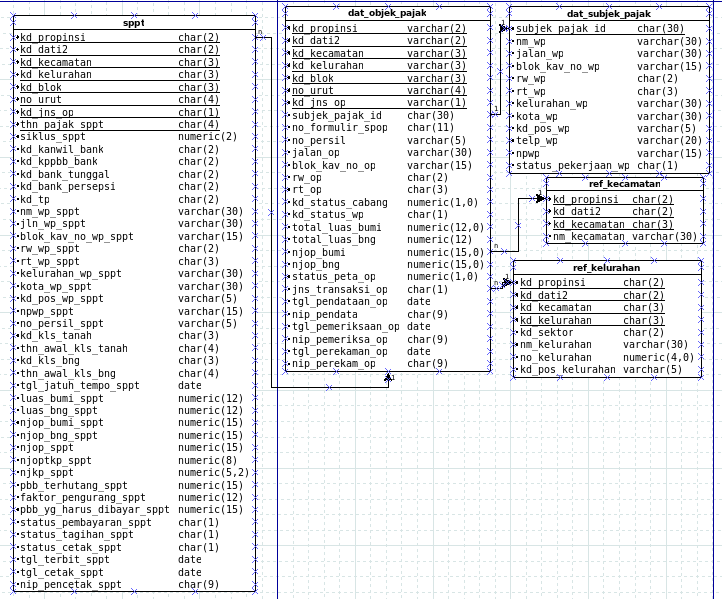
\includegraphics[width=1\textwidth]{./resources/db-diagram}
	\label{fig:diagram-relasi}
	\caption{Diagram Relasi \textit{Entity}}
\end{figure}

Titik utama akses aplikasi ini ada pada tabel \texttt{SPPT}, dimana nantinya tiap data pada tabel ini akan memiliki relasi n:1 dengan tabel \texttt{DAT\_OBJEK\_PAJAK}, ini karena tiap objek pajak yang tercatat akan memiliki banyak data SPPT untuk tiap tahun pajak.

Setiap data pada tabel \texttt{DAT\_OBJEK\_PAJAK} akan memiliki relasi 1:1 dengan data pada tabel \texttt{DAT\_SUBJEK\_PAJAK}.

Sedangkan hubungan atau relasi antara tabel \texttt{DAT\_OBJEK\_PAJAK} dengan \texttt{REF\_KECAMATAN} dan \texttt{DAT\_OBJEK\_PAJAK} dengan \texttt{REF\_KELURAHAN} adalah n:1, dimana tiap 1 (satu) data pada tabel \texttt{REF\_KECAMATAN} atau \texttt{REF\_KELURAHAN} akan memiliki banyak objek pada tabel \texttt{DAT\_OBJEK\_PAJAK}.

